\documentclass{article}
\usepackage[utf8]{inputenc}
\usepackage[italian]{babel}
\usepackage[T1]{fontenc}
\usepackage{tgpagella}
\title{
    Riconoscimento dello stato di una lavatrice \\
    \large Visione Artificiale e Riconoscimento
}

\author{Mara Pulighe - 001130145 \{mara.pulighe@studio.unibo.it\}\\
        Eugenio Tampieri - 001125222 \{eugenio.tampieri@studio.unibo.it\}}

\usepackage{natbib}
\usepackage{graphicx}

\begin{document}

\maketitle


\section{Introduzione al problema}\label{introduzione-al-problema}

\par Il problema affrontato consiste nell'individuazione automatica dello
stato della lavatrice (tempo residuo, fase e stato). Il sistema da noi
implementato mira a stabilire le basi per una soluzione robusta e
affidabile per il monitoraggio dei lavaggi.

\begin{figure}[h!]
  \centering
  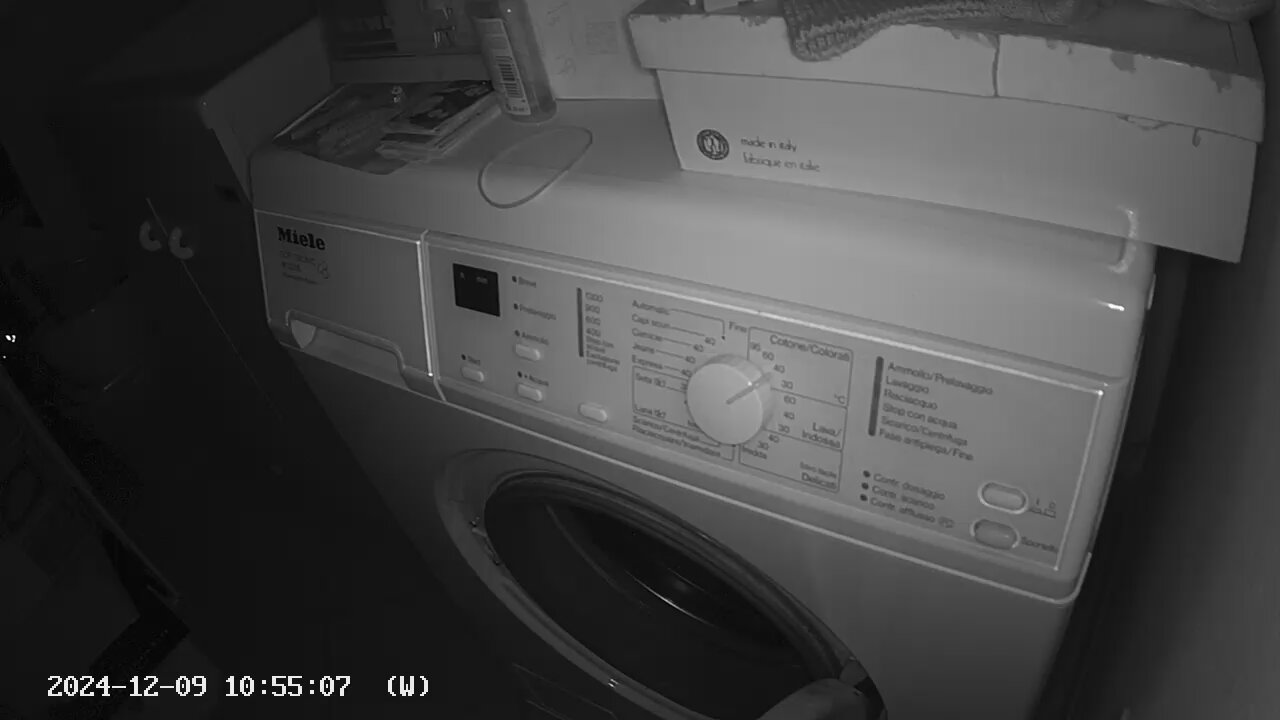
\includegraphics[scale=0.15]{1733738109}
  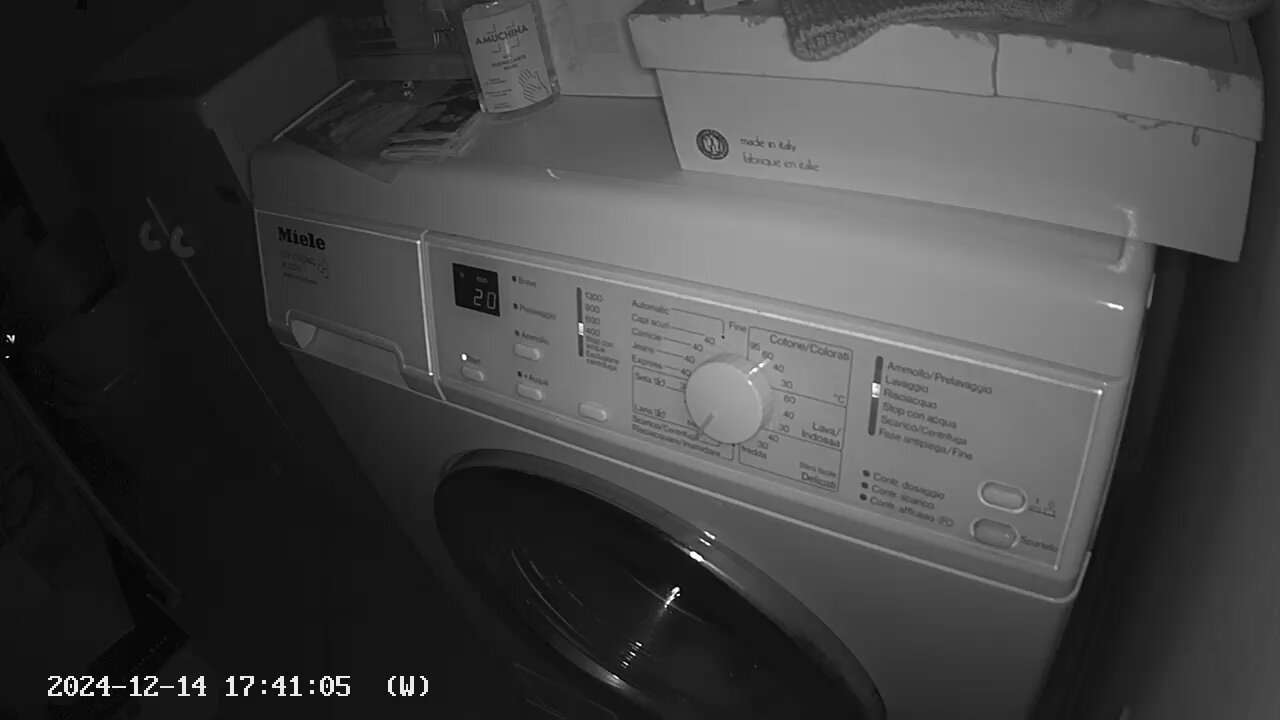
\includegraphics[scale=0.15]{1734194469R20}
  \caption{Due frame catturati dalla webcam, in cui la lavatrice è accesa e spenta.}
\end{figure}

\section{Stato dell'arte}\label{stato-dellarte}

\par Essendo il problema scomponibile in più sottoproblemi, lo stato
dell'arte va individuato separatamente per ognuno di essi.

\par Uno degli aspetti chiave del nostro sistema è l'individuazione dei
numeri che indicano il tempo rimanente per il completamento del ciclo di
lavaggio. Per questo compito, abbiamo utilizzato una rete neurale basata
su LeNet\citep{lecun2015lenet}. Le reti neurali convoluzionali (CNN) sono state ampiamente
utilizzate in applicazioni di visione artificiale e hanno mostrato
prestazioni superiori rispetto ai metodi tradizionali di riconoscimento
delle immagini.

\par Come visto in \textit{ImageNet} \citep{krizhevsky2012imagenet},
le CNN possono essere molto efficaci nel riconoscimento
delle immagini, aprendo la strada a molte applicazioni nel campo della
visione artificiale.

\par Per quanto riguarda invece il sottoproblema di riconoscimento della
fase, le tecniche tradizionali risultano essere in molti casi le
tecniche più semplici ed efficaci anche su problemi più complessi,
che quindi a loro volta utilizzano tecniche più complesse\citep{o2020deep}.

\section{Approccio sviluppato}\label{approccio-sviluppato}

\par Il nostro approccio combina l'uso di una rete neurale per il
riconoscimento dei numeri con l'analisi dell'intensità luminosa per
determinare lo stato della lavatrice.

\subsection{Reperimento del Dataset}\label{reperimento-del-dataset}

\par Attraverso una fotocamera fissa, in grado di inquadrare la parte
anteriore della lavatrice, sono state salvate circa due immagini al
minuto durante i diversi cicli di lavaggio e una al minuto quando la
lavatrice era in stato \textit{off}. È stato infatti elaborato un primitivo
algoritmo basato su regioni di interesse per determinare con sufficiente
precisione lo stato di alimentazione della lavatrice. Il salvataggio
delle immagini è stato impostato in modo che le immagini della lavatrice
in stato \textit{on} e \textit{off} venissero archiviate in cartelle separate
\footnote{Codice disponibile su https://github.com/eutampieri/washing-machine/blob/master/tools/on\_off\_detection/src/main.rs}.

\subsection{Individuazione delle Regioni di
Interesse}\label{individuazione-delle-regioni-di-interesse}

\begin{figure}[h!]
  \centering
  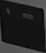
\includegraphics[scale=2]{display_template}
  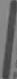
\includegraphics[scale=0.5]{template_bar}
  \caption{I template utilizzati per l'individuazione delle regioni.}
\end{figure}

\par Le due regioni rilevanti per trattare il problema sono quella del
display e quella della fase. Per farlo, abbiamo utilizzato la tecnica
del template matching\citep{jain2000statistical}\citep{hart2000pattern}, ricavando dei template da un'immagine con stato
\textit{off} dopo aver effettuato il pre-processing delle immagini. Il
problema è stato trattato come tre sotto-task: l'individuazione della fase,
la classificazione in acceso o spento e il riconoscimento delle cifre del display.

\subsection{Lavoro sui problemi}\label{lavoro-sui-problemi}

\par Abbiamo inizialmente lavorato su una singola immagine per comprendere
quali tecnologie utilizzare e poi generalizzato su tutto il dataset.
\par Nello specifico, abbiamo adottato questo approccio:

\begin{enumerate}
\item
  \textbf{Fase della Lavatrice}: Calcolando la media e la
  varianza delle varie immagini per contrastare l'effetto della
  variazione delle condizioni di illuminazione, viene binarizzata
  l'immagine. Dopodiché, tramite gli operatori morfologici, questa viene
  ripulita. Infine, viene individuata la regione accesa dell'immagine e
  viene mappata alla fase corrispondente.
\item
  \textbf{Lavatrice Accesa o Spenta}: La regione utilizzata è
  quella della fase. Viene utilizzato il risultato dell'analisi del
  primo task per classificare la lavatrice come accesa o spenta.
\item
  \textbf{Minuti Rimanenti al Completamento del Lavaggio}: Dopo
  aver estratto le singole cifre del display (tramite regioni definite
  all'interno di esso), viene eseguita l'inferenza su una rete da noi in
  precedenza addestrata basata su LeNet, alla quale abbiamo aggiunto un
  neurone di output per riconoscere il display spento. Questa rete ha
  dimostrato di essere efficace nel riconoscimento di numeri in
  immagini, anche se non siamo riusciti a renderla resistente agli
  spostamenti verticali\footnote{Aggiungendo del padding verticale,
  la rete raggiungeva fra il 60\% e il 70\%, e non si ottenevano dei
  buoni risultati aumentando il numero di epoche.}.
\end{enumerate}

\section{Valutazione sperimentale}\label{valutazione-sperimentale}

\par Per addestrare la rete neurale, abbiamo utilizzato l'accuratezza e la
loss come indicatori di prestazione, dopo aver suddiviso il dataset in
train, test e validation. Per valutare l'accuratezza dei singoli
sottoproblemi, abbiamo calcolato la percentuale di fasi e stati on/off
correttamente rilevati, mentre per quanto riguarda il problema del
riconoscimento dei minuti rimanenti abbiamo calcolato l'errore commesso
rispetto al valore contenuto nella label.

\par Abbiamo calcolato la media delle tre accuratezze ottenendo
un'accuratezza complessiva del sistema pari al 94,5\% (98,6
\% sul riconoscimento della fase, 92,8\% sui minuti rimanenti e 92,0\% su acceso/spento)

\par Durante le nostre analisi, abbiamo notato che la rete ha avuto
difficoltà a classificare correttamente l'ultima cifra del display. In
generale, riteniamo che gli errori siano legati alle regioni di
interesse selezionate, suggerendo che un'ulteriore ottimizzazione delle
aree analizzate potrebbe migliorare le prestazioni del sistema.

\section{Conclusioni e possibili sviluppi
futuri}\label{conclusioni-e-possibili-sviluppi-futuri}

\par In conclusione, il nostro lavoro ha dimostrato la fattibilità di un
sistema di monitoraggio delle fasi di lavaggio delle lavatrici
utilizzando tecniche di visione artificiale. Tuttavia, ci sono diverse
opportunità per migliorare ulteriormente il sistema.

\par Una possibile direzione futura potrebbe essere l'individuazione del
ciclo di lavaggio indicato dalla rotella, utilizzando tecniche basate
sulla trasformata di Hough. Inoltre, si potrebbe implementare una
soluzione meno sensibile agli spostamenti della fotocamera, per
garantire una maggiore robustezza del sistema. Infine, sarebbe utile
rendere il sistema più resistente alle variazioni di scala, in modo da
garantire prestazioni ottimali in diverse condizioni operative.

\par Inoltre, l'algoritmo sviluppato potrebbe essere integrato in un
sistema di domotica come HomeAssistant, ad esempio tramite MQTT.
\bibliographystyle{plain}
\bibliography{references}
\end{document}

